In this section we provide a general overview of different methodologies for computing the gradient/derivative of a loss function that includes the solution of differential equations. 
Without aiming at making an extensive and specialized review on the field, we find this resource useful for other researchers and students working on problems that combine optimization and sensitivity analysis with differential equations. 

Consider a system of ordinary differential equations given by
\begin{equation}
 \frac{du}{dt} = f(u, \theta, t),
 \label{eq:original_ODE}
\end{equation}
where $u \in \mathbb{R}^n$, $\theta \in \mathbb R^p$, and initial condition $u(t_0) = u_0$. 
Here $n$ denotes the total number of ordinary differential equations and $p$ the size of a parameter embedded in the functional form of the differential equation. 
Although we consider here the case of ordinary differential equations, that is, when the derivatives are just with respect to the time variable $t$, we will later include the case of partial differential equations (PDE).
We are interested in computing the gradient of a given loss function $L(u(\cdot, \theta))$ with respect to the parameter $\theta$. 
Examples of loss functions include
\begin{equation}
 L(u(\cdot, \theta)) = \| u(t_1, \theta) - u_1 \|_2^2,
\end{equation}
where $u_1$ is the desired target observation at some later time $t_1$; and
\begin{equation}
 L(u(\cdot, \theta)) = \int_{t_0}^{t_1} h( u(t;\theta), \theta) ) dt, 
\end{equation}
with $h$ some function that quantifies the contribution of the error term at time $t \in [t_0, t_1]$.
We are interested in computing the gradient of the loss function with respect to the parameter $\theta$, which can be written as
\begin{equation}
 \frac{dL}{d\theta} = \frac{dL}{du} \frac{du}{d\theta}.
 \label{eq:dLdtheta_VJP}
\end{equation} 
The first term is usually easy to evaluate, since it just involves the partial derivative of the scalar loss function to the solution. 
The second term on the right hand side is the actual bottleneck and it is usually referred to as the sensitivity,
\begin{equation}
 s = \frac{\partial u}{\partial \theta} \in \mathbb R^{n \times p}.
\end{equation}

\begin{figure}[]
    \centering
    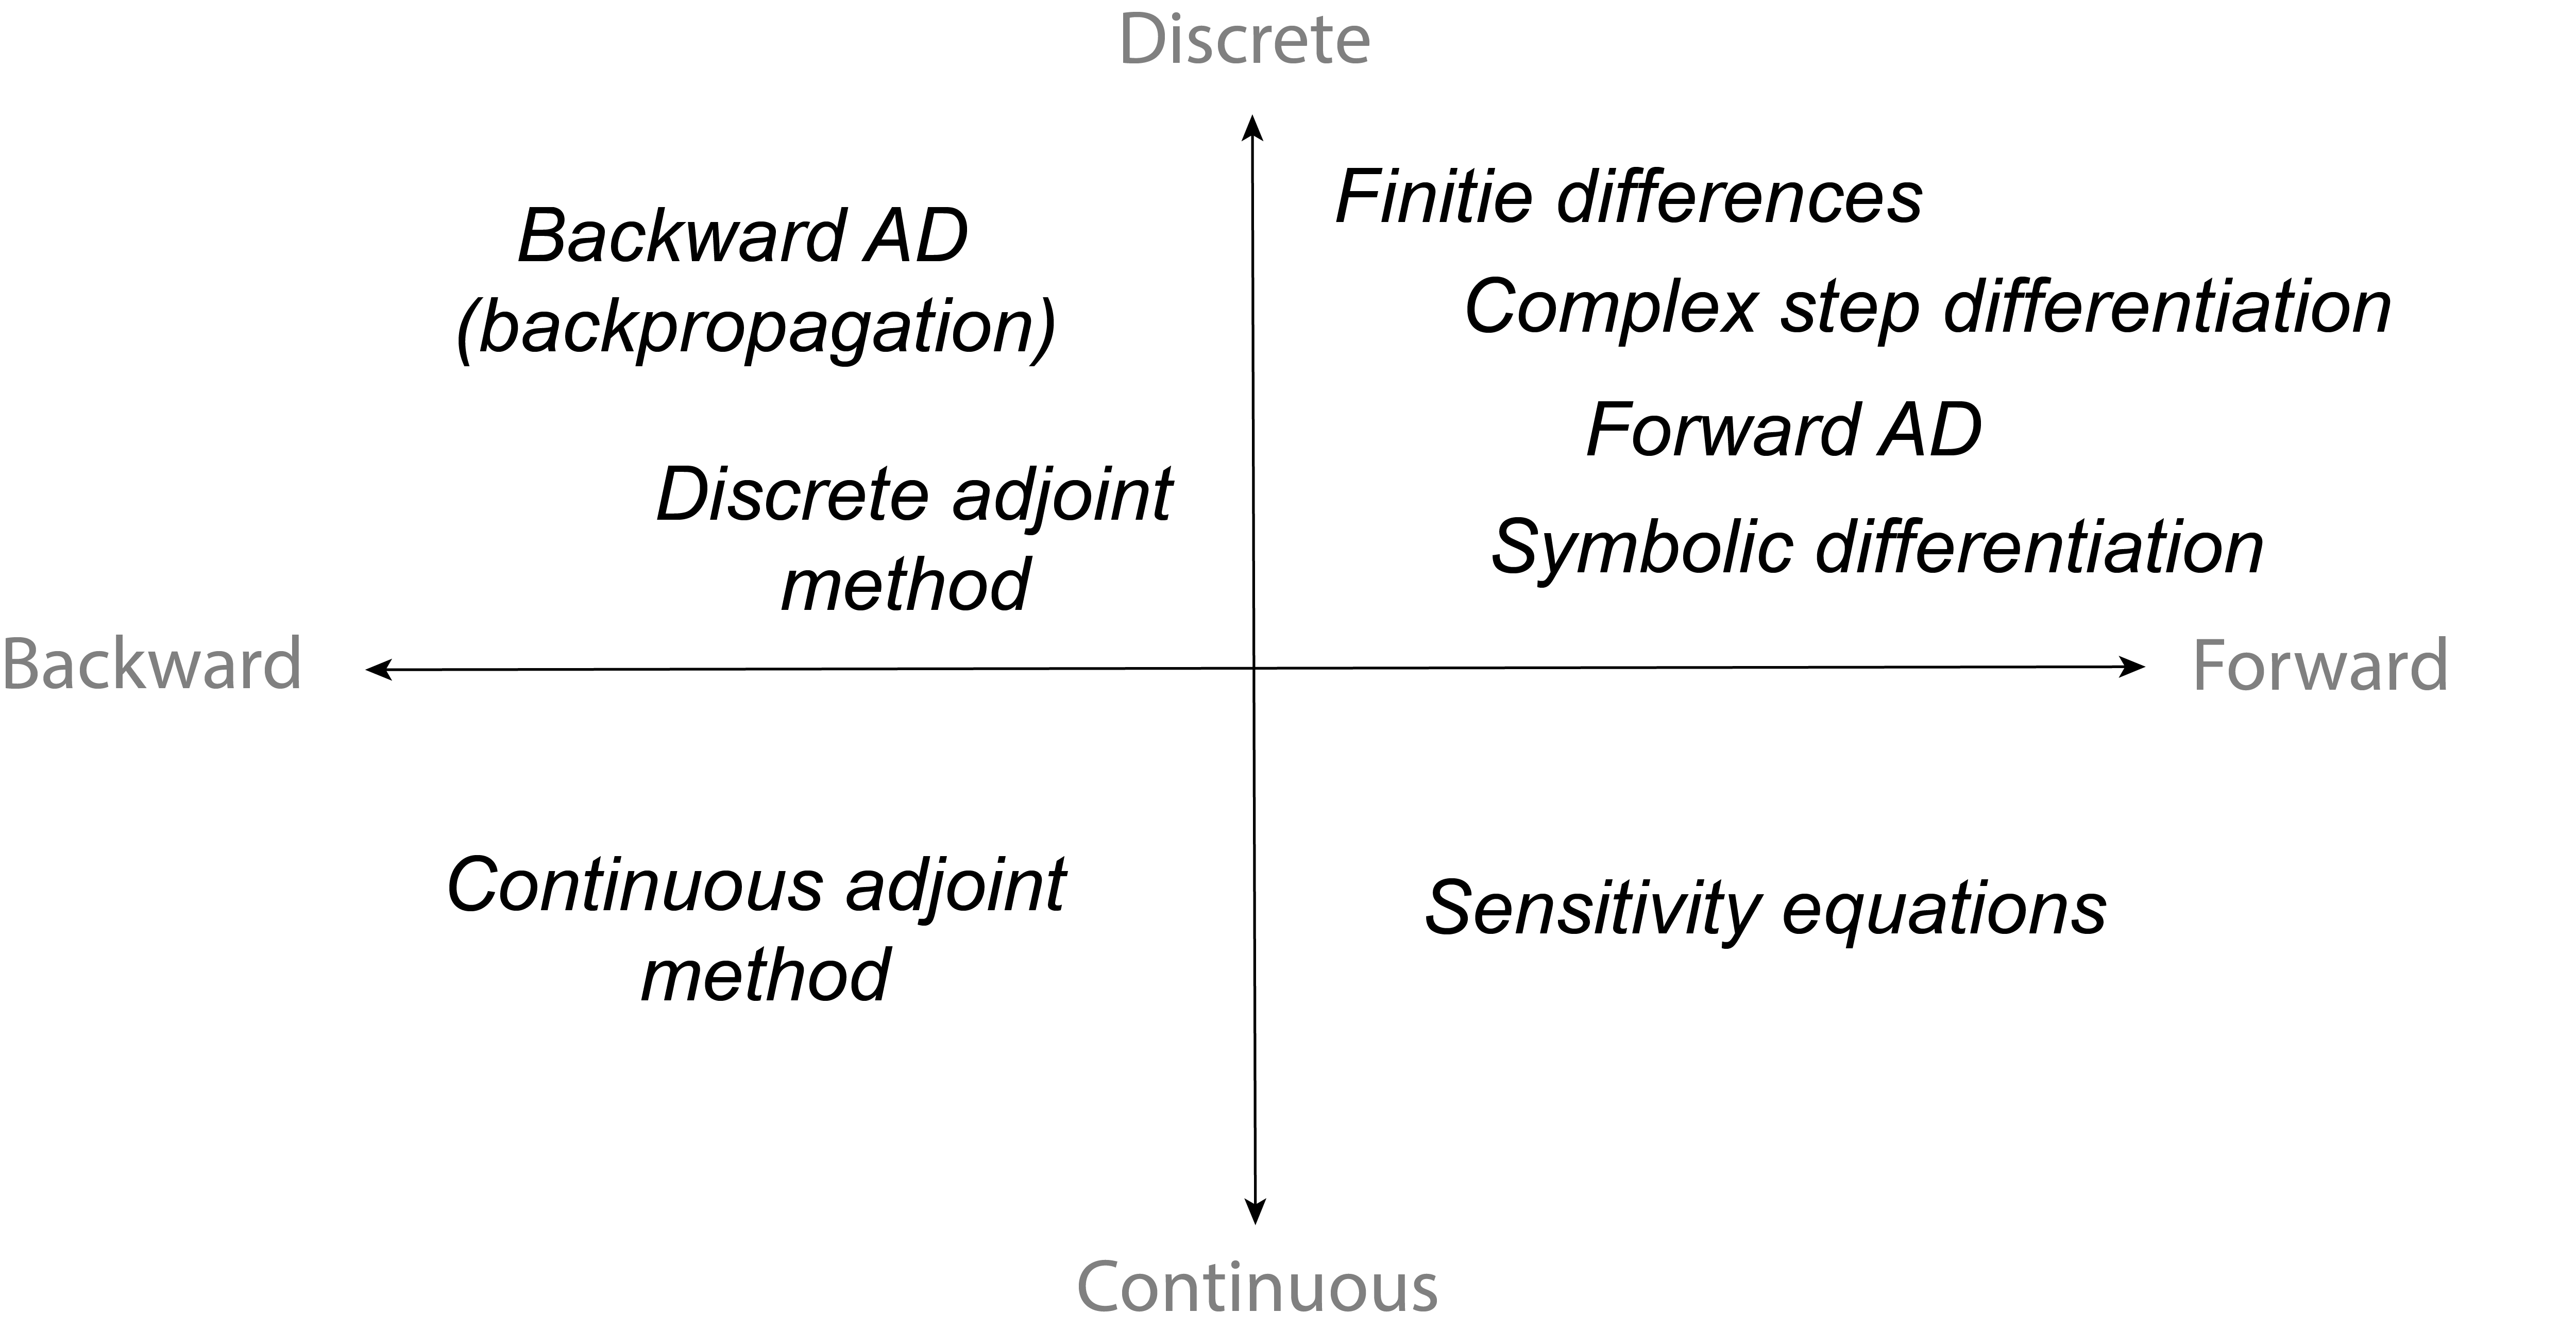
\includegraphics[width=0.80\textwidth]{figures/scheme-methods.png}
    \caption{Schematic representation of the different methods available for differentiation involving differential equation solutions.}
    \label{fig:diff}
\end{figure}
Depending on the number of parameters and the complexity of the differential equation we are trying to solve, there are different methods to compute gradients with different numerical and computational advantages and that also scale differently depending of the number of differential equations $n$ and number of parameters $p$. 
These methods can be roughly classified as:
\begin{itemize}
    \item \textit{Discrete} vs \textit{continuous} methods.
    \item \textit{Forward} vs \textit{backwards} methods.
\end{itemize}
The first difference regards the fact that the method for computing the gradient can be either based on the manipulation of atomic operations that are easy to differentiate using the chain rule several times (discrete), in opposition to the approach of approximating the gradient as the numerical solution of a new set of differential equations (continuous). 
The second distinction is related to the fact that some methods compute gradients by resolving a new sequential problem that may move in the same direction of the original numerical solver - i.e. moving forward in time - or, instead, they solve a new system that goes backwards in time. 
Figure \ref{fig:diff} displays a classification of some methods under this two-fold classification. In the following section we are going to explore more in detail these methods.